\documentclass[a4paper]{article}

\usepackage{geometry}
\geometry{left=1.5cm, right=1.5cm, top=2.54cm, bottom=2.54cm}
\usepackage{graphicx, hyperref, setspace, amsmath, amssymb, titlesec, fancyhdr, multicol, parskip, indentfirst, etoolbox, caption, cite, xcolor}
\usepackage{algorithm}
\usepackage{algpseudocode}
\usepackage{cuted}

\titleformat{\section}{\centering\large\scshape}{\thesection}{1em}{}
\titleformat{\subsection}{\normalsize\bfseries}{\thesubsection.}{1em}{}
\setstretch{1.0} 
\setlength{\parskip}{6pt} 
\titlespacing{\section}{0pt}{6pt}{6pt}
\titlespacing{\subsection}{0pt}{6pt}{6pt}
\titlespacing{\subsubsection}{0pt}{6pt}{6pt}

\title{Real-Time Localization Framework for Autonomous Basketball Robots}

\date{} 
\captionsetup{labelfont={small,sc}, textfont={small,sc}}

\renewcommand{\thesection}{\Roman{section}.}
\renewcommand{\thesubsection}{\textit{\Alph{subsection}.}}
\renewcommand{\thesubsubsection}{\textit{\arabic{subsubsection}.}}
\renewcommand{\thetable}{\Roman{table}} 
\renewcommand{\thefigure}{\Roman{figure}} 

\titleformat{\subsection}{\normalfont\large\itshape}{\thesubsection}{1em}{}
\titleformat{\subsubsection}{\normalfont\itshape}{\thesubsubsection}{1em}{}


\makeatletter
\renewcommand{\maketitle}{
  \begin{center}
    \noindent\rule{\textwidth}{1pt}\par
    \vspace{0.3em}
    {\LARGE \bfseries \@title \par}
    \vspace{0.3em}
    \noindent\rule{\textwidth}{1pt}\par
  \end{center}
}
\makeatother

\begin{document}

\maketitle
\vspace{1cm}


\begin{multicols}{2}
    \centering
    \textbf{Naren Medarametla}\\
    \textit{School of Computer Science Engineering}\\
    \textit{Vellore Institute of Technology}\\
    \textit{Chennai, India}\\
    \texttt{naren.medarametla2023@vitstudent.ac.in}
    \vfill\null

    \columnbreak

    \textbf{Sreejon Mondal}\\
    \textit{School of Electrical and Electronics Engineering}\\
    \textit{Vellore Institute of Technology}\\
    \textit{Chennai, India}\\
    \texttt{sreejon.mondal2023@vitstudent.ac.in}
    \vfill\null
\end{multicols}

\singlespacing
\setlength{\parskip}{6pt}
\setlength{\parindent}{0.5cm}

\begin{multicols}{2}
\setlength{\columnsep}{0.5cm}

\noindent \textbf{\textit{Abstract---}
Localization is a fundamental capability for autonomous robots, enabling them 
to operate effectively in dynamic environments. In Robocon 2025, accurate and 
reliable localization is crucial for improving shooting precision, avoiding 
collisions with other robots, and navigating the competition field efficiently. 
In this paper, we propose a hybrid localization algorithm that integrates classical 
techniques with learning-based methods, relying solely on visual data from the court’s
floor to achieve self-localization on the basketball field.
}

\small	
\noindent \textbf{
  \textit{Keywords---}\textit{Robot Localization, Autonomous Navigation, Neural Networks, Robocon}}

\section{Introduction}
\par \noindent
\textbf{Section II} reviews existing methods and prior research related to this work. 
\textbf{Section III} provides a detailed description of our proposed algorithm, approach, and model architecture. 
\textbf{Section IV} provides the results obtained from our experiments. 
\textbf{Section V} evaluates the accuracy of our approach and discusses potential directions for future work.


\section{Related Work}
%uently occur that pleasures have to be repudiated and annoyances accepted. The wise man therefore always holds in these matters to this principle of selection: he rejects pleasures to secure other greater pleasures, or else he endures pains to avoid worse pains
\section{Methodology}
\par \noindent Our approach is a two-step process that begins with \textbf{Preprocessing} the image,
followed by passing it to the model for \textbf{Inference}.
\subsection{Preprocessing}
\par \noindent The input image having dimensions (640 $\times$ 480 $\times$ 3) is converted from the RGB color space to the HSV color space, then the white regions are masked out using two predefined HSV ranges.
The image is downsampled through a radial scan, flattened, and finally passed through the neural network.

\par \noindent
% (TODO) also add labels in the paragarphs pointing to images and algorithms like figure a, etc
% fix image size and label size

{ \centering
  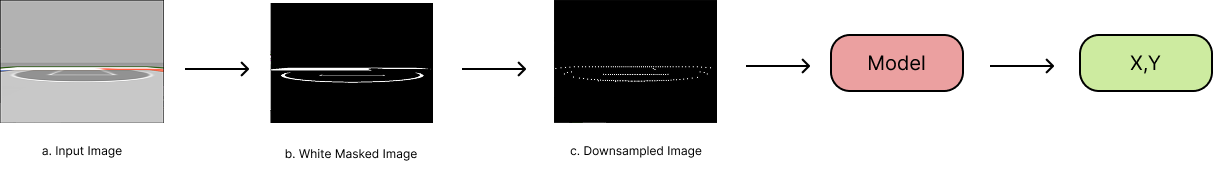
\includegraphics[width=0.5\textwidth]{../results/Flowchart.png}\\
  \captionof{figure}{preprocessing pipeline}\label{fig:flowchart}
}
\begin{algorithm}[H]
  \caption{Downsampling}
\begin{algorithmic}[1]
\Statex \textbf{Input: }Image
\State $H \gets$ Image.height
\State $W \gets$ Image.width
\State $R \gets$ Black Image
\For{angle $\gets$ 0 to 180 step 2}
    \State $lastPixel \gets 0$
    \State $cx \gets \text{W / 2}$
    \State $cy \gets \text{H}$
    \For{d $\gets$ 0 to max(H, W)}
        \State $x \gets cx + d \times \cos(angle)$
        \State $y \gets cy - d \times \sin(angle)$
        \If{$0 \leq x < \text{W} \ \textbf{and} \ 0 \leq y < \text{H}$}
          \State $pixel \gets Image[y][x]$
          \If{lastPixel = 255 and pixel $\neq$ 255}
            \State $R[y][x] \gets 255 $ 
          \EndIf
          \State $lastPixel \gets pixel$
        \EndIf
    \EndFor
\EndFor
\State \textbf{Return} R
\end{algorithmic}
\end{algorithm}

\subsection{Model Architecture}
\par \noindent
The proposed model is a feedforward neural network consisting of a flattening layer followed 
by four fully connected layers. The first 200 pixels from the top of the image are removed 
to reduce the input size, as they do not carry useful information.

\par \noindent
The resulting image with dimensions (640 $\times$ 280 $\times$ 1) is flattened into a vector 
of size 1,79,200 and passed through the first linear layer, followed by a ReLU activation function.
The subsequent layers have sizes 1024, 256, and 64, each followed by a ReLU activation. 
The final layer outputs a 2-dimensional vector representing the predicted $x$ and $y$ positions of the robot.

\par \noindent
The rationale for using this relatively simple model lies in the simplicity of the input images 
and to reducing inference time.

%maybe could add input dimensions for each layer??
{ \centering
 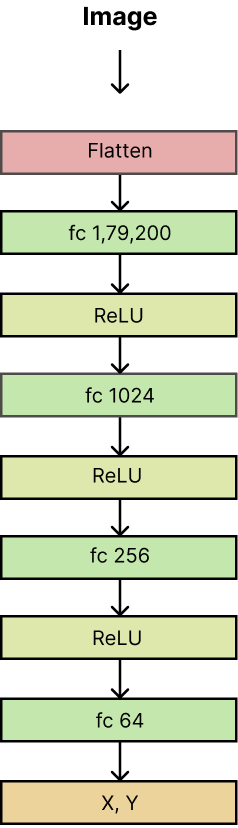
\includegraphics[width=0.2\columnwidth]{../results/model.png}\\
 \captionof{figure}{architecture diagram}\label{pinki}
}

%write about figure number which shows the architecture

% write about dataset collection and gazebo simulation
% also write about training the model, epochs, optimiser, cost fn, batch size, etc

\subsection{Dataset} 

\par \noindent
A digital twin of the robot was created and simulated in a replica of the Robocon 2025 arena 
using the Gazebo \cite{gazebo} simulator with the help of ROS 2 \cite{macenski2022ros2}. 

\par \noindent
The robot was driven through the arena capturing images and corresponding $x$, $y$ coordinates. A 
TimeSynchronizer was used to synchronize the frame header and the position header. A total of
6283 images were captured and split into training  and test datasets with a 0.9 to 0.1 ratio.
Care was taken to include every part of the arena for an unbiased dataset. 

% attach gazebo picture here as well

\subsection{Training}
\par \noindent
The model was trained for 15 epochs using an Adam optimizer \cite{kingma2014adam} with an initial learning rate of $10^{-4}$
and a Mean Squared Error (MSE) loss function. 

\section{Results and Analysis}
% add repo link as well
\section{Conclusion}  % write about future work as well

\begin{thebibliography}{99}

\bibitem{gazebo}
N. Koenig and A. Howard, "Design and use paradigms for Gazebo, an open-source 
multi-robot simulator," 2004 IEEE/RSJ International Conference on Intelligent Robots 
and Systems (IROS) (IEEE Cat. No.04CH37566), Sendai, Japan, 2004, pp. 2149-2154 vol.3, 
doi: 10.1109/IROS.2004.1389727.
  
\bibitem{macenski2022ros2}
Steve Macenski, Tully Foote, Brian Gerkey, Chris Lalancette, and William Woodall. 
\textit{Robot Operating System 2: Design, architecture, and uses in the wild}. 
Science Robotics, vol. 7, no. 66, 2022. 

\bibitem{kingma2014adam}
Diederik P. Kingma and Jimmy Ba. 
\textit{Adam: A method for stochastic optimization}. 
arXiv preprint arXiv:1412.6980, 2014.

\end{thebibliography}

\end{multicols}

\end{document}